\documentclass{article}

\usepackage{caption}
\usepackage{subcaption}

\usepackage[margin=1in]{geometry}
\usepackage{custom}

\title{Measuring the Distance to Pluto with Nickel Astrometry \\ ASTR 257: Observational Astronomy}
\author{Aditya Sengupta}

\begin{document}
    \maketitle
    \section{Observations}

    We planned observations of Pluto with the Direct Imaging Camera on the Nickel telescope at Lick Observatory. The instrument has a field of view of 6.3 $\times$ 6.3 arcseconds and is subdivided into a grid of 2048$\times$2048 pixels. We selected 2x binning in order to improve read noise while ensuring the signal-to-noise ratio was sufficiently high to observe the target, making the plate scale of the instrument 0.368 px/arcsec. We planned on taking science images with a 10 s integration time, subject to saturation or low counts. Accordingly, we took dark current frames at 5 s and 10 s integration times, along with bias frames and flat-field frames. We took five of each type of calibration frame.

    Due to poor weather conditions on the scheduled nights, data from the 2019 iteration of this class, taken by Arcelia Hermosillo Ruiz, were used for reductions and results. These data were taken at UT 2019-09-23 03:07:47 through 03:13:38 on the first night, and 2019-09-24 03:05:02 through 03:10:35 on the second. At the start of observing on the first night, the coordinates of Pluto were RA 19h28m32.30s and Dec -22d24m27.1s. The data were taken using a V filter and 2x binning, and the science frames were taken at a 30 s integration time.

    \section{Reductions}

    The raw frames were dark-subtracted (adjusting for the exposure time of the darks) and flat-fielded. Since the flat-field images were taken on sky at twilight, the earlier frames had higher levels of background illumination than the later ones. In order to compensate for this, we take the pixel-by-pixel median of the biases, darks, and flats, and further normalize by dividing each by their overall median across the whole image. This removes a brightness gradient across the uncalibrated images. 

    \begin{figure}
        \centering
        \begin{subfigure}[b]{0.45\textwidth}
            \centering
            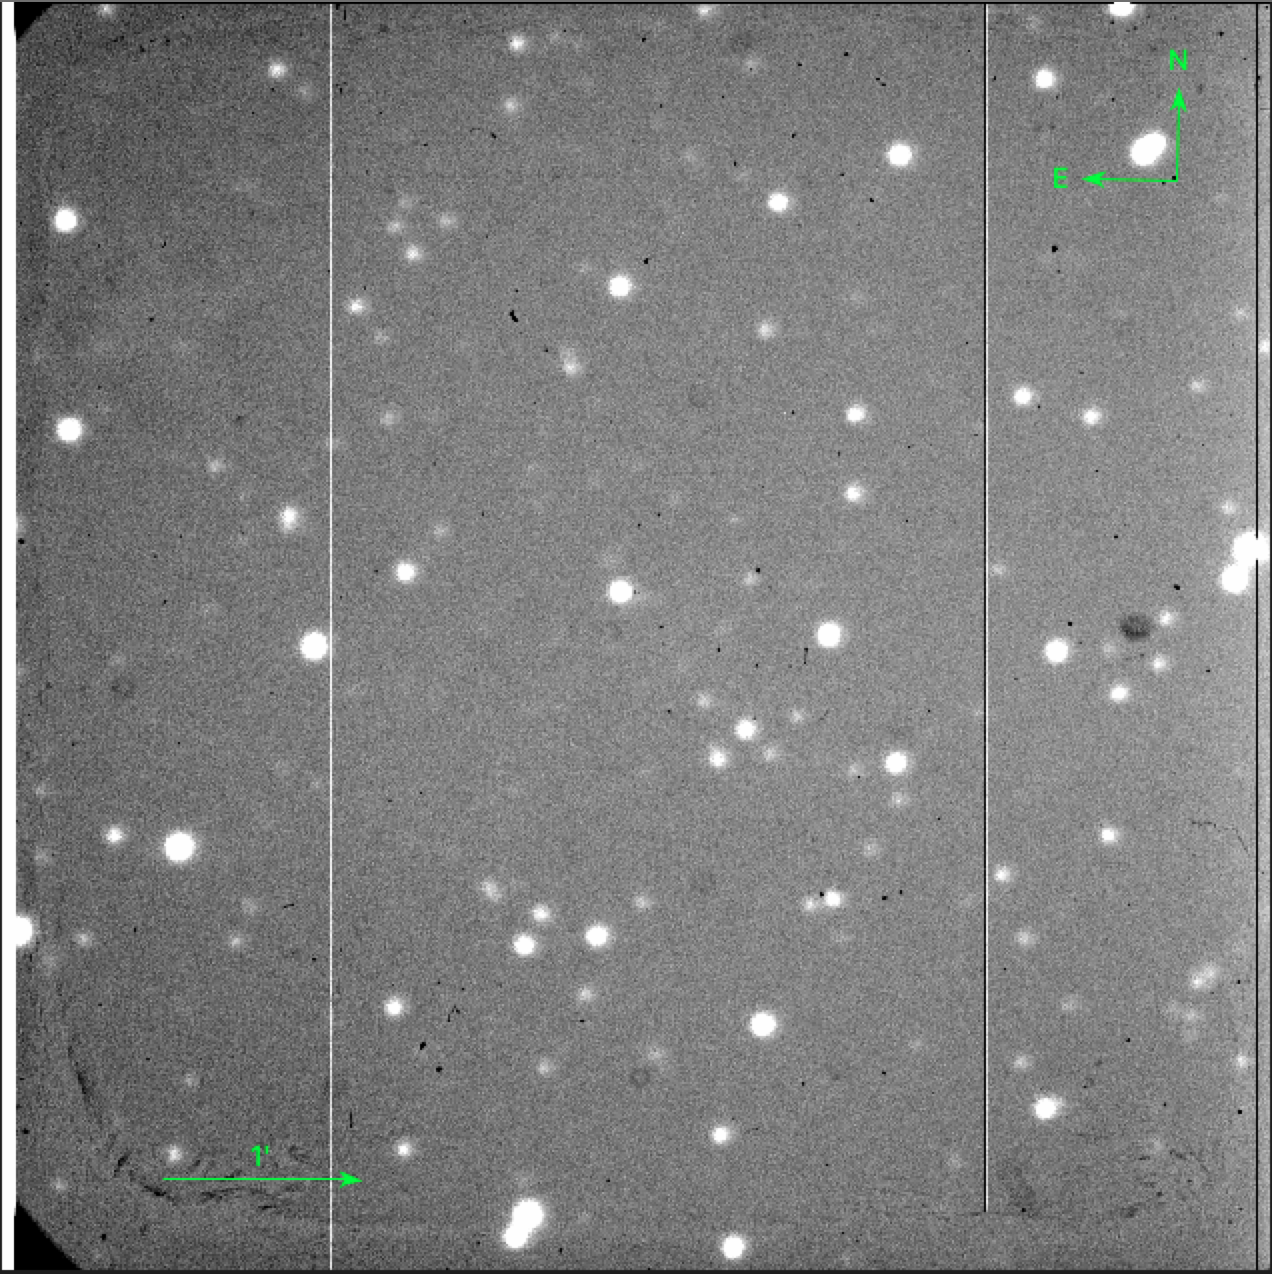
\includegraphics[width=\textwidth]{sci1.png}
            \caption{First night}
            \label{fig:sci1}
        \end{subfigure}
        \hfill
        \begin{subfigure}[b]{0.45\textwidth}
            \centering
            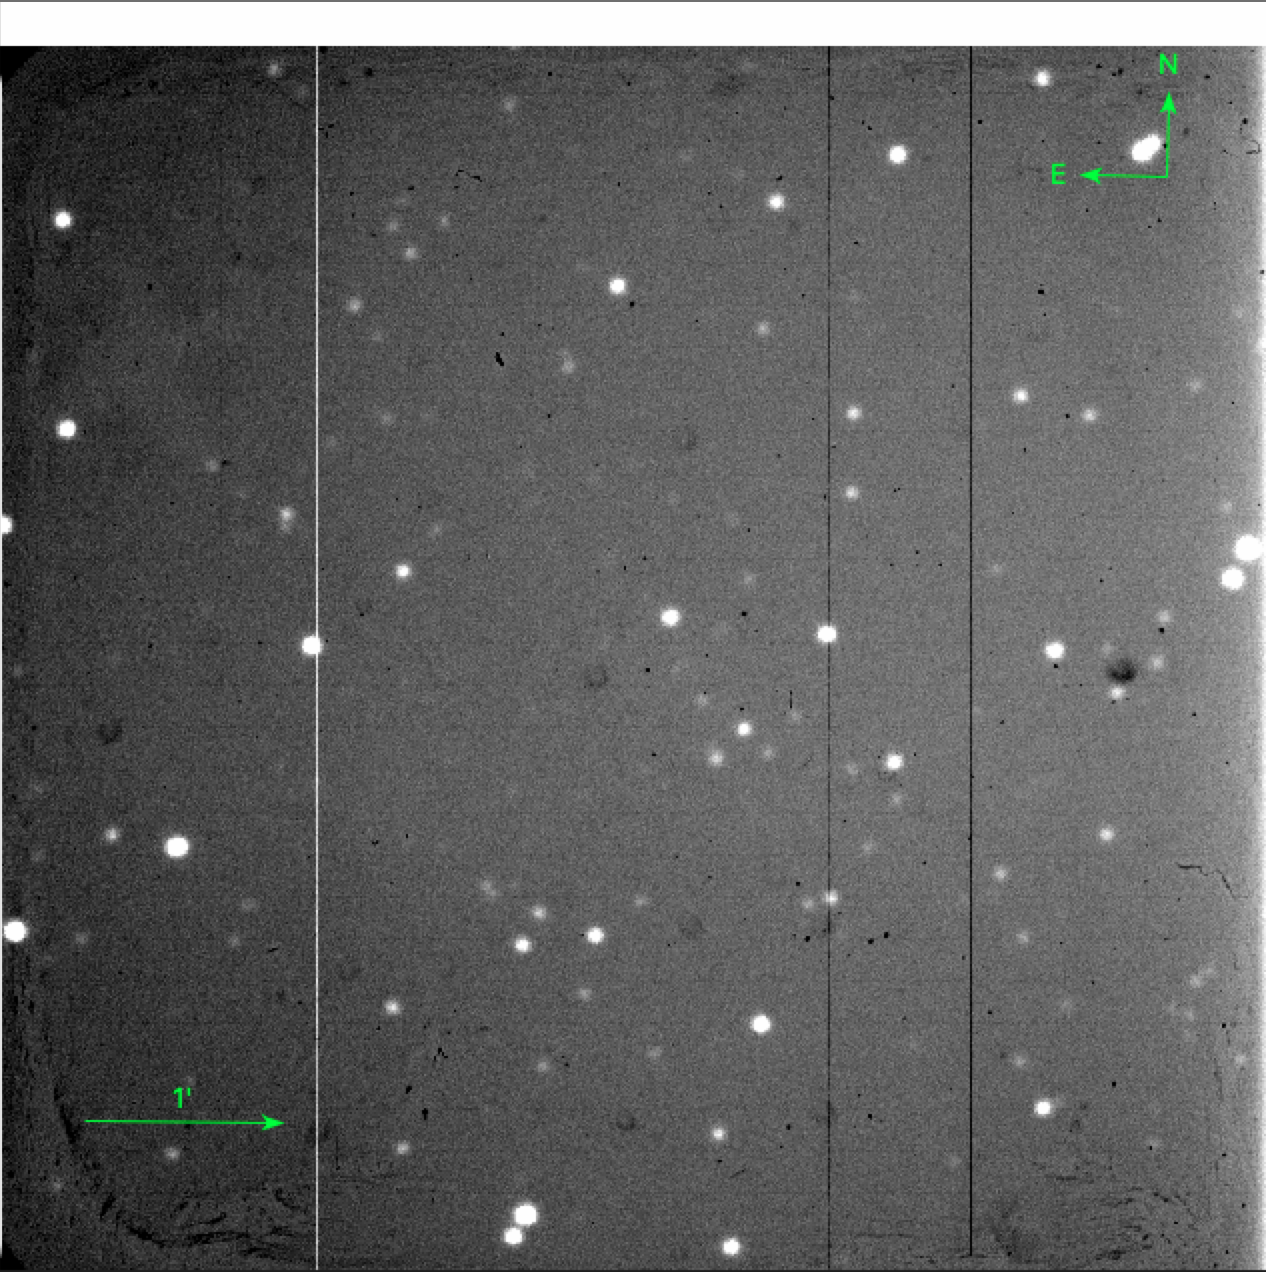
\includegraphics[width=\textwidth]{sci2.png}
            \caption{Second night}
            \label{fig:sci2}
        \end{subfigure}
           \caption{Calibrated science images from both nights.}
           \label{fig:science}
   \end{figure}

   Due to slightly different telescope pointings between the two nights, there was an offset between the two calibrated images. This was adjusted by isolating a 200x200 px cutout of both images with just one distinct source, finding its centroid in both images using the \textit{photutils} Python package, and shifting the image by the offset calculated between the two images of this source. The shift was 35 pixels in the $x$ direction and -10 pixels in the $y$ direction. By blinking between the two offset images in ds9, we confirmed the background had been correctly adjusted and the only visible motion was that of Pluto. Figure~\ref{fig:science} shows the calibrated and offset images on both nights. 

    \section{Results}

    By taking \textit{photutils} centroids on the appropriate cutout around Pluto on both nights, we found that Pluto moved by 46.52 px between the two images. We converted the pixel offset to arcseconds using the Nickel plate scale of 0.184 arcsec/pixel, and multiplied the result by 2 to account for the binning. We found the offset in astronomical coordinates to be 17.17 arcseconds. This is approximately equal to the value measured by the scale tool in ds9.

    Assuming coplanar circular orbits and that Pluto's movement over a single night is dwarfed by Earth's, we can compute the distance from Earth to Pluto using this measurement. 

    \begin{figure}
        \centering
        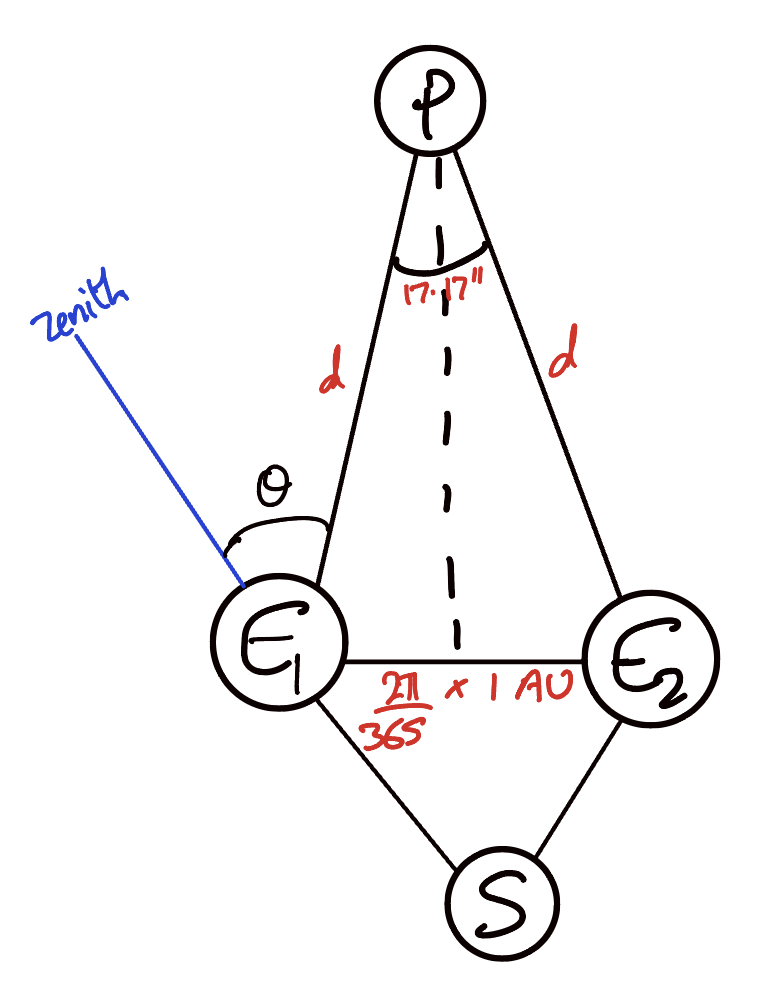
\includegraphics[width=0.4\textwidth]{pluto_arc.jpeg}
        \caption{Diagram of the Sun-Earth-Pluto system. The desired distance $d$ can be computed from the measured angle and the known movement of the Earth over one day.}
        \label{fig:pluto_arc}
    \end{figure}
    
    Figure~\ref{fig:pluto_arc} shows the relative positions of Earth on the two nights and Pluto. Using this, we find 

    \begin{align}
        \sin\frac{17.17"}{2} \approx \frac{\frac{2\pi}{365} \cdot \frac{1}{2}\text{AU}}{d/cos\theta} \implies \frac{d}{\cos\theta} \approx 209 \text{AU}.
    \end{align}

    We multiply a corrective factor that relaxes the assumption that Pluto is at opposition. We assume the N-S line overhead at midnight is at 0 hours RA (as the measurement was taken the day after September 21) meaning the angle between zenith and Pluto was approximately 4h32m, or 68 degrees. Therefore the corrective factor we multiply is $\cos\theta = \cos(68^\circ) \approx 0.375$, meaning the true distance estimate is $d = 78.3 \text{AU}$.

    Pluto's distance from the Sun is between 30 and 49 AU, meaning while it is observable, we should have an Earth-Pluto distance of no more than 49 AU. To resolve this discrepancy, we look at the assumptions we made. Earth's orbit has an eccentricity of around 0.016, meaning over a single night the assumed distance it moved relative to the Sun is not significantly different than the considered value. The remaining discrepancy could be addressed by dropping the assumption that Pluto does not move between the two nights.
\end{document}